%%----------------------------------------------------------------------------
%% Onderzoekstechnieken: Een bachelorproefvoorstel schrijven
%%----------------------------------------------------------------------------

\documentclass[aspectratio=169]{beamer}

%==============================================================================
% Aanloop
%==============================================================================

%---------- Vormgeving --------------------------------------------------------

\usetheme{hogent}

\usecolortheme{hgwhite} % witte achtergrond, zwarte tekst

\usepackage{graphicx,multicol}
\usepackage{comment,enumerate,hyperref}
\usepackage{amsmath,amsfonts,amssymb}
\usepackage[english]{babel}
\usepackage{multirow}
\usepackage{eurosym}
\usepackage{listings}
\usepackage{textcomp}
\usepackage{framed}
\usepackage{wrapfig}
\usepackage{tabu} %needed for \tabulinesep
\usepackage{wrapfig}
\usepackage{pgf-pie}
\usepackage{pgfplots}
\usepackage{booktabs}
\usepackage{pgfplotstable}
\usepackage{changepage}
\usepackage{ulem} % for \sout{text} (strikethrough)
\usepackage{fancyvrb} % for \begin{Verbatim} (LaTeX controls within verbatim)

%---------- Configuratie ------------------------------------------------------

\pgfplotsset{compat=1.16}
\usetikzlibrary{arrows,shapes,backgrounds,positioning,shadows,calc}
\usetikzlibrary{pgfplots.statistics}

%---------- Commando-definities -----------------------------------------------

\newcommand{\tabitem}{~~\llap{\textbullet}~~}
\newcommand{\alertbox}[2][hgblue]{%
  \setbeamercolor{alertbox}{bg=#1,fg=white}
  \begin{beamercolorbox}[sep=2pt,center]{alertbox}
    \textbf{#2}
  \end{beamercolorbox}
}
\pgfmathdeclarefunction{gauss}{2}{%
  \pgfmathparse{1/(#2*sqrt(2*pi))*exp(-((x-#1)^2)/(2*#2^2))}%
}

%---------- Bibliografie ------------------------------------------------------

\usepackage[backend=biber,style=apa]{biblatex}
\DeclareLanguageMapping{dutch}{dutch-apa}
\addbibresource{ozt-oef-1-latex.bib}

%---------- Info over de presentatie ------------------------------------------

\title{Writing a Research Report}
\subtitle{Research Techniques}
\author{Jens Buysse \and Pieter-Jan Maenhaut \and Bert {Van Vreckem}}
\date{AY 2020-2021}

%==============================================================================
% Inhoud presentatie
%==============================================================================

\begin{document}

\begin{frame}
  \maketitle
\end{frame}

\begin{frame}
  \frametitle{What's on the menu?}
  
  \tableofcontents
\end{frame}


\section{How to report on research?}

\subsection{Stages in writing}

\begin{frame}
  \frametitle{Stages in writing}
  \centering
  \begin{tikzpicture}[
  auto,
  thick,
  ->,
  >=stealth',
  shorten >=1pt,
  node distance=1.2cm,
  fase/.style={ shape=rectangle, fill=hgblue!30, draw}]
  
  \node[fase] (1) {Planning};
  \node[fase] (2) [below of=1] {Structure};
  \node[fase] (3) [below of=2] {Draft Version};
  \node[fase] (4) [below of=3] {Design};
  \node[fase] (5) [below of=4] {Revision};
  
  \draw (1) -- (2);
  \draw (2) -- (3);
  \draw (3) -- (4);
  \draw (4) -- (5);
  \end{tikzpicture}
\end{frame}

\begin{frame}
  \frametitle{Planning the document}
  
  \begin{description}
    \item[Why?] Objective
    \item[Who?] Who is your audience? Adjust writing style and level!
    \item[What?] Contents: outline or mind map
    \item[When?] Take time constraints into account, make planning
    \item[Where?] Environment
    \item[Tools?] Which tools, software? Install them!
  \end{description}
\end{frame}

\begin{frame}
  \frametitle{The audience}
  
  \begin{columns}[c]
    \column{.5\textwidth}
    
    \centering
    
    \textbf{The specialist}
    
    
\includegraphics[height=3cm]{oef2-04.png}
    
    \begin{itemize}
      \item Want to see many details
      \item Knows technical terms
    \end{itemize}
    
    \column{.5\textwidth}
    
    \centering
    
    \textbf{The non-specialist}
    
    
\includegraphics[height=3cm]{oef2-05}
    
    \begin{itemize}
      \item More background, interpretation needed
      \item Non-technical terms required
      \item Want to see technical terms explained
    \end{itemize}
  \end{columns}
\end{frame}

\begin{frame}
  \frametitle{The audience: some tips}
  
  Technical terms vs. slang
  
  \begin{itemize}
    \item Technical terms: specific to the discipline, you can clarify
    \item Slang: laziness, wanting to impress
  \end{itemize}
  
  \vfill
  
  \centering
  
  \textcolor{hgorange}{$\times$ The PS3 has 6 $\times$ SPE @3.2GHz}
  
  vs.
  
  \textcolor{hgdarkgreen}{$\checkmark$ The Playstation 3 has 6 \textbf{Synergistic Processing Elements} at a clock speed of 3.2 GHz.}
\end{frame}

\begin{frame}
  \frametitle{The audience: some tips}
  
  \begin{itemize}
    \item Explain abbreviations
    \item Use list of abbreviations if necessary (and make sure it containts all abbreviations!)
  \end{itemize}
  
  \vfill \centering
  
  \textbf{IP =}
  
  Internet Protocol?
  
  Intellectual Property?
  
  Interpersonal?
  
  In Progress?
  
  etc.
  
  (\url{http://www.acronymfinder.com/IP.html})
  
\end{frame}

\begin{frame}
  \frametitle{The audience: some tips}
  
  Add conclusions explicitly (separate section)
  
  \begin{itemize}
    \item Often read first
    \begin{itemize}
      \item Billboard of your work!
    \end{itemize}
    \item Even though your audience can draw conclusions themselves
    \begin{itemize}
      \item This does not mean they will
      \item Other interpretations possible
      \item You are the specialist, not them
    \end{itemize}
  \end{itemize}
\end{frame}

\subsection{Document Structure}

\begin{frame}[plain]
  \frametitle{Document structure}
  
  \begin{columns}
    \column{.5\textwidth}
    \begin{center}
      Traditional approach:
      
      \begin{tikzpicture}[auto,thick,->,>=stealth',
      shorten >=1pt, node distance=2.3cm,
      fase/.style={shape=rectangle,inner sep=8pt,fill=hgorange,draw}]
      
      \node[fase] (1) {Approach};
      \node[fase] (2) [below of=1] {Results};
      \node[fase] (3) [below of=2] {Conclusions};
      
      \draw (1) -- (2);
      \draw (2) -- (3);
      
      \end{tikzpicture}
    \end{center}
    \column{.5\textwidth}
    \begin{center}
      Selective approach:
      
      \begin{tikzpicture}[auto,thick,->,>=stealth',
      shorten >=1pt, node distance=2.3cm,
      fase/.style={shape=rectangle,inner sep=8pt,fill=hgdarkgreen,draw}]
      
      \node[fase] (1) {Conclusions};
      \node[fase] (2) [below of=1] {Results};
      \node[fase] (3) [below of=2] {Approach};
      
      \draw (1) -- (2);
      \draw (2) -- (3);
      
      \end{tikzpicture}
    \end{center}
  \end{columns}
\end{frame}

\begin{frame}
  \frametitle{Workflow $\ne$ text order}
  
  Readers are interested in motivation and conclusions of your work, generally not in the details of your approach.
  
  \vfill
  
  \begin{columns}
    \column{.25\textwidth}
    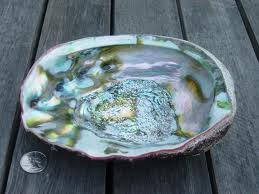
\includegraphics[width=\textwidth]{oef2-06}
    
    \column{.75\textwidth}
    \begin{quotation}
      Inspired by an abalone shell, Angela Belcher programs viruses to make elegant nanoscale structures that humans can use. Selecting for high-performing genes through directed evolution, she’s produced viruses that can construct powerful new batteries, clean hydrogen fuels and record-breaking solar cells.
    \end{quotation}
  \end{columns}
\end{frame}

\begin{frame}
  \frametitle{Document structure}
  \framesubtitle{Short document}
  
  \begin{columns}
    \column{.5\textwidth}
    \centering
    \begin{tikzpicture}[auto,thick,
    deel/.style={shape=rectangle,fill=hgdarkgreen,
      minimum width=4cm,draw}
    ]
    
    \node[deel] (1) [minimum height=24pt] {Introduction};
    \node[deel] (2) [below=6pt of 1,minimum height=56pt,fill=hgblue] {Corpus/body};
    \node[deel] (3) [below=6pt of 2,minimum height=24pt] {Conclusions};
    
    \end{tikzpicture}
    
    \column{.5\textwidth}
    \centering
    \begin{tikzpicture}[auto,thick,
    deel/.style={ shape=rectangle,fill=hgdarkgreen,
      minimum width=4cm,draw}]
    
    \node[deel] (1) [minimum height=24pt] {Preface};
    \node[deel] (2) [below=6pt of 1,minimum height=24pt] {Summary};
    \node[deel] (3) [below=6pt of 2,minimum height=56pt,fill=hgblue] {Corpus/body};
    \node[deel] (4) [below=6pt of 3,minimum height=24pt] {Conclusions};
    
    \end{tikzpicture}
    
  \end{columns}
\end{frame}

\begin{frame}[plain]
  \frametitle{Document structure}
  \framesubtitle{Long document}
  
  \begin{columns}
    \column{.5\textwidth}
    \centering
    \begin{tikzpicture}[auto,thick,
    deel/.style={ shape=rectangle,fill=hgdarkgreen,
      minimum width=4cm,draw}]
    
    \node[deel] (1) [minimum height=24pt] {Abstract};
    \node[deel] (2) [below=6pt of 1,minimum height=24pt] {Introduction};
    \node[deel] (3) [below=6pt of 2,minimum height=56pt,fill=hgblue] {Corpus/body};
    \node[deel] (4) [below=6pt of 3,minimum height=24pt] {Conclusions};
    \end{tikzpicture}
    
    \column{.5\textwidth}
    \centering
    \begin{tikzpicture}[auto,thick,
    deel/.style={ shape=rectangle,fill=hgdarkgreen,
      minimum width=4cm,draw}]
    
    \node[deel] (1) [minimum height=24pt] {Preface};
    \node[deel] (2) [below=6pt of 1,minimum height=24pt] {Summary};
    \node[deel] (3) [below=6pt of 2,minimum height=24pt] {Introduction};
    \node[deel] (4) [below=6pt of 3,minimum height=56pt,fill=hgblue] {Corpus/body};
    \node[deel] (5) [below=6pt of 4,minimum height=24pt] {Conclusions};
    \end{tikzpicture}
    
  \end{columns}
\end{frame}

\begin{frame}
  \frametitle{Document structure}
  
  Preface
  
  \begin{description}
    \item[Context] Why is this work important?
    \item[Need] Why did this need to be investigated?
    \item[Task] What did you do in the end?
    \item[Object] What is written in this document?
  \end{description}
  
  Summary (abstract)
  
  \begin{description}
    \item[Result] Contents of this work?
    \item[Conclusion] Relevance for the public
    \item[Perspective] Future work?
  \end{description}
  
  (short document = 1 paragraph, long document = max. ~1 page)
\end{frame}

\begin{frame}[plain]
  %\frametitle{Voorbeeld voorwoord/samenvatting (abstract)}
  
  \begin{center}
    \only<1>{Context}
    \only<2>{Need}
    \only<3>{Task}
    \only<4>{Object}
    \only<5>{Result+Conclusion}
  \end{center}
  
  \scriptsize
  \textbf{Energy-Efficient Resource Provisioning Algorithms for Optical Clouds}
  
  \alert<1>{Rising energy costs and climate change have led to an increased concern for energy-efficiency (EE).} \alert<2>{As Information and Communication Technology (ICT) is responsible for about 4\% of total energy consumption worldwide, it is essential to devise policies aimed at reducing it.} \alert<3>{In this paper, we propose a routing and scheduling algorithm for a cloud architecture, which targets minimal total energy consumption by enabling switching off unused network and/or Information Technology (IT) resources, exploiting the cloud-specific anycast principle.} \alert<4>{A detailed energy model for the entire cloud infrastructure comprising wide area optical network and IT resources is provided. This model is used to make a single-step decision on which IT end points to use for a given request, including the routing of the network connection towards these end points. Our simulations quantitatively assess the EE algorithm’s potential energy savings, but also assess the influence this may have on traditional Quality of Service parameters such as service blocking. Furthermore, we compare the one-step scheduling with traditional scheduling and routing schemes, which calculate the resource provisioning in a two-step approach (selecting first the destination IT end point, and subsequently using unicast routing towards it).} \alert<5>{We show that depending on the offered infrastructure load, our proposed one step calculation considerably lowers the total energy consumption (reduction up to 50\%) compared to the traditional iterative scheduling and routing, especially in low to medium load scenarios, without any significant increase in the service blocking.}
  
\end{frame}

\section{How to refer to professional literature?}

\subsection{Why a literature review?}

\begin{frame}
  \frametitle{Common mistakes}
  
  \begin{itemize}
    \item Incomplete / no references
    \item Only URLs
    \item Missing information in references
    \begin{itemize}
      \item $\Rightarrow$ sources cannot be found
    \end{itemize}
    \item Unacceptable sources
    \item Wrong layout
    \item No references to sources from text
    \item Broken down by type (book, web, etc.)
  \end{itemize}
\end{frame}

\begin{frame}
  \frametitle{Purpose of the literature review}
  
  \begin{itemize}
    \item Introduction to subject
    \item What is the current state of the art?
    \item What do experts say about this topic?
    \item Clarify research questions, place them in context
    \item There is a problem that requires a solution
  \end{itemize}
  
  \bigskip
  
  \alertbox{\textcolor{hgyellow}{Every statement} in a literature review must be proven by using a reference}
\end{frame}

\begin{frame}
  \frametitle{Purpose of the reference list}
  
  Allow readers to:
  
  \begin{itemize}
    \item Look up the referenced sources
    \item Evaluate the value of sources themselves
  \end{itemize}
  
  \pause
  
  Strict, pre-defined format:
  
  \begin{itemize}
    \item Pre-defined rules, depending on publication (e.g. IEEE, APA, Chicago Manual or Style, \ldots)
    \item Fixed order (order in the text or alphabetically)
    \item List of URLs is insufficient!
  \end{itemize}
  
  \pause
  
  \alertbox{Use \textcolor{hgyellow}{reference management software} to create your reference list!}
\end{frame}

\begin{frame}
  \frametitle{When to refer to literature?}
  
  \begin{itemize}
    \item Definitions, first introduction of technical term
    \item Copy from source of literal quote, translation/paraphrase, or image
    \begin{itemize}
      \item No reference = \alert{plagiarism!}
    \end{itemize}
    \item Cite the results of a previous study
    \item Almost every statement you make regarding the field
  \end{itemize}
  
  \bigskip
  
  \alertbox{References add \textcolor{hgyellow}{credibility} to your literature study}
\end{frame}

\subsection{Look up and track information}

\begin{frame}
  \frametitle{Types of sources}
  
  \begin{description}
    \item[Primary] Knowledge that you \textbf{acquire yourself} during research 
      
      Experiments, surveys, interviews, \ldots

    \item[Secondary] \textbf{Publication} of knowledge, research, \ldots by others
    
    Article in scientific or professional journal, presentation at conference, book, \ldots

    \item[Tertiary] \textbf{Indexes}

    Search engine, encyclopedia, library database, \ldots

  \end{description}
  
  \alertbox{Only \textcolor{hgyellow}{secondary sources} can be used as reference.}
\end{frame}

\begin{frame}
  \frametitle{Look up information}
  
  Start with \alert{tertiary} sources:
  
  \begin{itemize}
    \item Google Scholar: \url{https://scholar.google.com/}
    \item ScienceDirect: \url{https://www.sciencedirect.com/}
    \item Springer Online Journals: \url{https://link.springer.com/}
    \item Catalog Library: \url{https://www.hogent.be/student/bibliotheken/}
    \item Wikipedia (obviously\dots)
  \end{itemize}
  
  \alertbox{Please note: tertiary sources, in particular Wikipedia, are \textcolor{hgyellow}{not} acceptable as reference}
  
  \pause
  
  \begin{itemize}
    \item No guarantee on accuracy
    \item Claims not always demonstrated: [citation needed]
    \item But they \alert{are} a good starting point (e.g. references at bottom)
  \end{itemize}
\end{frame}

\begin{frame}
  \frametitle{Tips}
  
  \begin{itemize}
    \item<+-> Visit website HOGENT \textbf{library}: \url{https://www.hogent.be/student/bibliotheken/}
    \begin{itemize}
      \item Search, Theses / Tasks, Databases
      \item Information skills course (\url{https://chamilo.hogent.be/index.php?go=CourseViewer\&application=Chamilo\%5CApplication\%5CWeblcms\&course=22068\&tool=LearningPath\&browser=Table\&tool_action=ComplexDisplay\&publication=980981})
    \end{itemize}
    \item<+-> \textbf{Apollox} (\url{https://apollox.hogent.be/})
    \begin{itemize}
      \item launch applications/search engines from HoGent
      \item e.g.~SPSS, Endnote, Visio, Office
      \item Online journals and ebooks for which HoGent has a subscription (bv.~ScienceDirect, SpringerLink)
    \end{itemize}
  \end{itemize}
\end{frame}

\begin{frame}
  \frametitle{Tips (cont.)}
  
  \begin{itemize}
    \item<+-> \textbf{Google Scholar}
      \begin{itemize}
        \item Access from campus or via Apollo
        \item Look for download links on the right: [PDF] or [fulltext@Hogent]
        \item Reference in Bib{\TeX}-format (settings)
        \item Use search options (e.g.~limit search in time)
      \end{itemize}
    \item Presentations \textbf{conferences} (via Youtube, Vimeo, Slideshare, \dots)
    \begin{itemize}
      \item e.g. Google IO, WWDC, FOSDEM, Velocity, \dots
      \item Search via Lanyrd (\url{http://lanyrd.com/topics/})
    \end{itemize}
    \item<+-> Technical \textbf {portal sites} for ICT related topics
    \begin{itemize}
      \item e.g.~dzone.com, infoq.com, TechNet, enz.
    \end{itemize}
  \end{itemize}
\end{frame}

\begin{frame}
\frametitle{Tips (cont.)}

\begin{itemize}
    \item<+-> What are the most important names in the \ textbf {community}?
    \begin{itemize}
      \item Keynotes at conferences, authors of standard works, etc.
      \item Follow them on Twitter
      \item Search for their blogs
    \end{itemize}
    \item<+-> \textbf{Technical blogs} of companies
    \begin{itemize}
      \item Google Developers Blog, Twitter Engineering/Developer Blog, Netflix Tech Blog, \dots
    \end{itemize}
  \end{itemize}
\end{frame}


\begin{frame}
  \frametitle{Usable sources}
  
  (For a Bachelor thesis in Computer Science)
  
  \begin{description}
    \item[Journal article]<+-> in a scientific peer-reviewed journal
    \item[Conference proceedings]<+-> paper presented at a scientific, peer-reviewed congress
    \item[Thesis]<+-> doctorate (PhD), Master, possibly ~Bachelor
    \item[Manual]<+-> e.g.~of used or discussed software
    \item[Book]<+-> note: anyone can publish a book. Check author, publisher, target audience (Springer vs. ``for dummies'')
    \item[Presentation]<+-> by recognized expert, e.g. at conference (via Youtube, Vimeo, etc.)
    \item[Blogpost]<+-> if written by recognized expert
    \item[Trade Journal]<+-> note: written by journalist (is not an expert)
  \end{description}
\end{frame}

\begin{frame}
  \frametitle{Unusable sources}
  
  \begin{itemize}
    \item Any work without an author or publication year
    \item Wikipedia article
    \item Blog article from someone outside the field
    \item ``White papers'' (generally not objective)
    \item Homepage of a discussed product or company
    \begin{itemize}
      \item if needed add in text or as a footnote
    \end{itemize}
    \item \dots
  \end{itemize}
\end{frame}

\begin{frame}
  \frametitle{Checklist quality sources}
  \framesubtitle{Take the CRAP test}
  
  \begin{description}
    \item[Current] Publication year? Is it sufficiently recent? Is this still in accordance with the \textbf{state-of-the-art}?
    \item[Reliable] Is it objective? Balanced or one-sided?
    Citations?
    \item[Authoritative] Author? Is this a recognized expert? Referred to elsewhere?
    \item[Purpose/Point of View] Opinion or facts? Does the author want to sell something? Is it relevant to your research question?
  \end{description}
  
\end{frame}

\begin{frame}[fragile]
  \frametitle{Citation and reference list in {\LaTeX}}
  
  Bib{\LaTeX} and Biber
  
  \vspace{18pt}
  
  \verb|article.tex|: Main text\\
  \verb|article.bib|: Bibliographic database (edit with e.g.~JabRef)
  
  \vspace{18pt}
  
  Preamble:
  
  \begin{verbatim}
  \usepackage[backend=biber,style=apa]{biblatex}
  \DeclareLanguageMapping{dutch}{dutch-apa}
  \addbibresource{artikel.bib}
  \end{verbatim}
  
\end{frame}

\begin{frame}
  \frametitle{Bibliographic data in Jabref}
  
  Info that is \textbf{always} required:
  
  \begin{description}
    \item[Author] Last name, First name and Last name, First name and Last name, First name\ldots
    \item[Title] of the article, book, \ldots
    \item[Year] or date of publication
    \item[Bibtexkey] id of the source, used for citing (tip: click the key icon)
  \end{description}
\end{frame}

\begin{frame}[fragile]
  \frametitle{Bibliographic data in Jabref}
  \framesubtitle{Additional info for Article}
  
  \begin{description}
    \item[Journal] Name of the magazine
    \item[Volume] 
    \item[Number] Number within the volume (optional)
    \item[Pages] \verb|mmm--nnn|
  \end{description}

  \bigskip
  
  \textbf{Example:}
  
  \bigskip
  
  \fullcitebib{Anscombe1973}
\end{frame}

\begin{frame}
  \frametitle{Bibliographic data in Jabref}
  \framesubtitle{Additional info for Electronic}
  
  \begin{description}
    \item[Url] Hyperlink to source
    \item[Urldate] Date of consultation
  \end{description}

  \bigskip

  \textbf{Example:}

  \bigskip

  \fullcitebib{Lundin2020}

\end{frame}

\begin{frame}
  \frametitle{Bibliographic data in Jabref}
  \framesubtitle{Additional info for InProceedings}
  
  \begin{description}
    \item[Booktitle] ``Proceedings of the [conference name]''
    \item[Editor] Editor(s) (optional)
    \item[Pages] page numbers (optional)
  \end{description}
  
  \medskip
  
  \textbf{Example:}
  
  \fullcitebib{vanderLaanEtAl2015}
\end{frame}

\begin{frame}
  \frametitle{Bibliographic data in Jabref}
  
  Enter as much info as possible (facilitates searching):
  
  \begin{description}
    \item[DOI] Digital Object Identifier: unique ID for article, with this you can automatically fill in all fields
    \item[URL] even when it is not really an electronic source
    \item[Keywords] 
    \item[File] PDF of publication
    \item[Abstract] Summary
    \item[Comments] Your own summary/remarks
  \end{description}
  
\end{frame}

\begin{frame}[fragile]
  \frametitle{Source acknowledgment and reference list in {\LaTeX}}
  
  \begin{itemize}
    \item References in text:
    
    \begin{itemize}
      \item \verb|\textcite{Knuth1998}| $\Rightarrow$ Knuth (1998)
      \item \verb|\autocite{Knuth1998}| $\Rightarrow$ (Knuth, 1998)
    \end{itemize}
    
    \item Insert reference list: \verb|\printbibliography|
    
    \item Compile (using TexStudio):
    
    \begin{enumerate}
      \item Build/Compile (F5 of F6): references not added yet, ``keys'' are indicated in bold
      \item Bibliography (F8): selects the referenced sources and prepares them
      \item Build/Compile (F5 of F6): insert references and reference list effectively
    \end{enumerate}
  \end{itemize}
  
  Refer to the provided templates or the syllabus for examples!
\end{frame}

\begin{frame}
  \frametitle{Exercise}
  
  \begin{itemize}
    \item Compile the Research Techniques syllabus in TexStudio and check whether you can insert the bibliography and references 
    (F5 - F8 - F5)
    \item Find a number of articles related to the subject of the group task
    \item Add them to JabRef
    \begin{itemize}
      \item Keep as much information as possible (also e.g. abstract, keywords, PDF, URL)
    \end{itemize}
    \item Add text with references and reference list to the template of the article
  \end{itemize}
\end{frame}

\begin{frame}
  \frametitle{Additional information}
  
   Additional information and examples are available in the ``Praktische gids voor de bachelorproef''
  
  \vspace{12pt}
  
  \url{https://github.com/HoGentTIN/bachproef-gids/releases}
  
\end{frame}

\end{document}